%%------------------------------------------			
%\begin{frame} \frametitle{Syndromes and decoding}
%%-----------------------------------------------------			
%\vspace*{-0.25in}
%\begin{figure}[t]
%			\centering
%            \resizebox{4.0in}{!}{\begin{tikzpicture}

%A matrix
\draw [fill=cyan, opacity=.2,rotate=90, thick]  (0.1,4.35) node (v1) {} rectangle (3.9,-3.75) node (v2) {};
\draw [thick,rotate=90,red] (v1) rectangle (3.9,3.1);
\draw [thick,rotate=90,red] (0.1,3.1) rectangle (3.9,1.8) node (v7) {};
\draw [thick,rotate=90,red] (0.1,-2.45) node (v6) {} rectangle (v2);
\draw[thick,red]  (v6) rectangle (1.15,3.9);
\draw[thick,red]  (v7) rectangle (-0.55,0.1);

\node at (-0.45,-1.4) {\huge \color{red} $ \underset{ \color{blue} ( Parity  \ checks)}{H_{ m \times n} }$};

% X vector
\draw [ thick] (5.85,5) rectangle (6.85,6);
\draw [thick] (6.85,5) rectangle (5.85,4);
\draw [thick] (5.85,4) rectangle (6.85,3);
\draw [] (5.85,3) node (v4) {} rectangle (6.85,-0.1) node (v5) {};
\draw [thick] (5.85,-0.1) rectangle (6.85,-1.1);
\draw [thick] (5.85,-1.1) rectangle (6.85,-2.1) node (v8) {};
\node at (6.45,-3.4) {\huge \color{red}  $\underset{\tiny \color{blue} (code \ vector)}{c_{n \times 1 }} $};
\node at (6.35,1.6) {\Large \bf \vdots};

\draw [thick] (v4) rectangle (6.85,2.1);
\draw [thick] (v5) rectangle (5.85,0.8);

% delta-x vector
\draw [ thick, fill=green] (9.4,5) rectangle (10.4,6);
\draw [thick] (10.4,5) rectangle (9.4,4);
\draw [thick, fill=green] (9.4,4) rectangle (10.4,3);
\draw [] (9.4,3) node (v4) {} rectangle (10.4,-0.1) node (v5) {};
\draw [thick, fill=green] (9.4,-0.1) rectangle (10.4,-1.1);
\draw [thick] (9.4,-1.1) rectangle (10.4,-2.1);
\node at (10,-3.4) {\huge \color{red}  $\underset{\color{black}{t-sparse}}{\underset{\tiny \color{blue} (error \ vector)}{e}} $};
\node at (9.9,1.6) {\Large \bf \vdots};
\node at (4.8,2.1) {\bf \Huge $\times$};
\draw [thick] (v4) rectangle (10.4,2.1);
\draw [thick] (v5) rectangle (9.4,0.8);

\node at (8.2,2) {\Huge \bf $+$};

\node at (9.9,5.5) {\color{red} \huge $ e_i$ };
\node at (9.9,3.5) {\color{red} \huge $ e_j$};
\node at (9.9,-0.55) {\color{red} \huge $ e_t$};

% y







\node at (15.9,1.6) {\bf \vdots};

\node at (11.8,2) {\Huge = };
\node at (15.8,-0.65) {\color{red} \huge $y_{m \times 1}$};
\node [align=left, text width =3.5cm] at (16.5,-2.15) {\Large  \color{blue} Syndromes};

\node at (0.3,2.45) {\Huge \bf $\cdots$};



% b_k

\draw [thick] (15.4,4.1) node (v3) {} rectangle (16.4,3.1);
\draw [thick] (15.4,3.1) rectangle (16.4,2.1);
\draw [thick] (15.4,2.1) rectangle (16.4,1);
\draw [thick] (15.4,1) rectangle (16.4,0);
\draw[fill=red, opacity=0.2]  (v3) rectangle (16.4,0);
\node at (-1.35,1.6) { \color{blue}\Large  \bf  \vdots};

\draw [dashed,blue] (-4.35,3.9) rectangle (3.75,3);
\draw [dashed,blue] (-4.35,3) rectangle (3.75,2);
\draw[dashed,blue]  (v1) rectangle (3.75,1);
\node at (-3.85,4.5) {\huge \bf  \color{red} $h_1$};
\node at (-2.4,4.5) {\huge \bf \color{red} $h_2$};
\node at (-1.25,4.5) {\huge \bf  \color{red} $h_i$};
\node at (0.25,4.5) {\huge \bf  \color{red} $\cdots$};
\node at (1.8,4.5) {\huge \bf  \color{red} $h_{n-1}$};
\node at (3.15,4.5) {\huge \bf  \color{red} $h_n$};

\node at (9.9,4.55) {\large \bf \vdots};


\node at (13.45,2) {\bf \Huge $0$};
\node at (14.45,2) {\huge \bf +};

\draw [fill=orange, opacity=0.5] (v8) rectangle (5.85,6);
\end{tikzpicture} }
%			%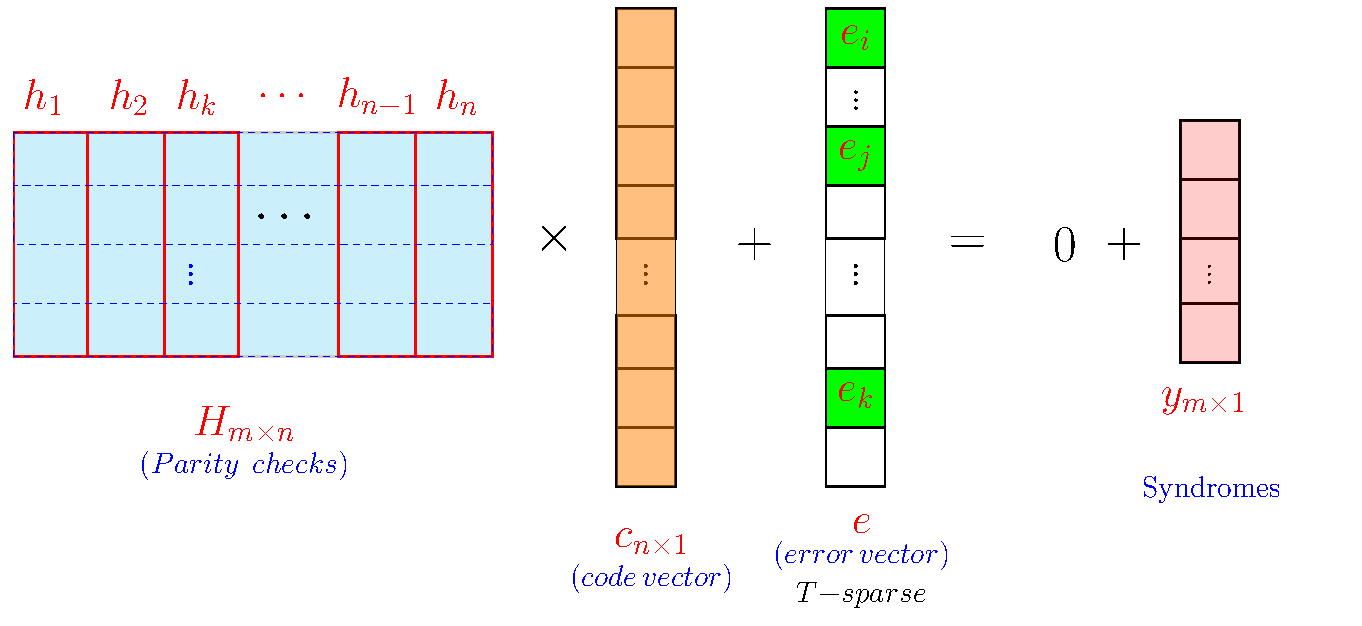
\includegraphics[width=4.0in]{./Figures/A_times_X_columns_coding.pdf}
%		\end{figure}
%\pause
%\begin{itemize}
%\item Syndrome : Linear combination of $\underline{h}_i$s, i.e., $\underline{y} = e_i \hv_i \oplus e_j \hv_j \oplus e_t \hv_t$
%\item Decoding : Find min weight $\underline{e}$ : $\underline{y} = e_i \hv_i \oplus e_j \hv_j \oplus e_t \hv_t$
%\end{itemize}
%\pause
%\begin{block}{\alert{Coding theory deals with the construction of $\mathbf{H}$ and efficient decoding algorithms, i.e., given a linear combination of the columns of $\mathbf{H}$, it develops tools to determine a sparse $\underline{e}$ }}\end{block}
%\end{frame}
%%------------------------------------------			
%\begin{frame} \frametitle{Syndrome source coding}
%%\begin{block}{Compression of a $p-$ary source}
%%\[
%%\begin{bmatrix}
%%y_1\\
%%\vdots\\
%%y_m\\
%%\end{bmatrix}
%%=
%%\begin{bmatrix}
%%  1 & 1 & 1 & \ldots & 1 \\
%%  1 & W & W^2 & \ldots & W^{n-1} \\
%%  1 & W^2 & W^4 & \ldots & W^{2n-2} \\
%%  \vdots & \vdots & \vdots & \vdots & \vdots \\
%%  1 & W^{2t-1} & W^{4t-2} & \ldots & W^{(2t-1)(n-1)}\\
%%\end{bmatrix}
%%\begin{bmatrix}
%%0\\
%%\vdots\\
%%x_1\\
%%\vdots \\
%%x_{k}\\
%%\vdots\\
%%0\\
%%\end{bmatrix}
%%\]
%%\end{block}
%
%\resizebox{4.0in}{!}{\begin{tikzpicture}

%A matrix
\begin{scope}[shift={(2,0)}]
\draw [fill=cyan, opacity=0.2,rotate=90, thick]  (0.1,4.35) node (v1) {} rectangle (3.9,-3.75) node (v2) {};
\draw [thick,rotate=90,red] (v1) rectangle (3.9,3.1);
\draw [thick,rotate=90,red] (0.1,3.1) rectangle (3.9,1.8) node (v7) {};
\draw [thick,rotate=90,red] (0.1,-2.45) node (v6) {} rectangle (v2);
\draw[thick,red]  (v6) rectangle (1.15,3.9);
\draw[thick,red]  (v7) rectangle (-0.55,0.1);
\node at (-0.45,-1.4) {\huge \color{red} $ \underset{ \color{blue} ( Parity  \ check \ matrix )}{H_{ m \times n} }$};
\node at (4.8,2.1) {\bf \Huge $\times$};
\node at (0.3,2.45) {\Huge \bf $\cdots$};
\node at (-1.35,1.6) { \color{blue}\Large  \bf  \vdots};
\draw [dashed,blue] (-4.35,3.9) rectangle (3.75,3);
\draw [dashed,blue] (-4.35,3) rectangle (3.75,2);
\draw[dashed,blue]  (v1) rectangle (3.75,1);
\node at (-3.85,4.5) {\huge \bf  \color{red} $h_1$};
\node at (-2.4,4.5) {\huge \bf \color{red} $h_2$};
\node at (-1.25,4.5) {\huge \bf  \color{red} $h_i$};
\node at (0.25,4.5) {\huge \bf  \color{red} $\cdots$};
\node at (1.8,4.5) {\huge \bf  \color{red} $h_{n-1}$};
\node at (3.15,4.5) {\huge \bf  \color{red} $h_n$};

\end{scope}










% X vector
%\draw [ thick] (5.85,5) rectangle (6.85,6);
%\draw [thick] (6.85,5) rectangle (5.85,4);
%\draw [thick] (5.85,4) rectangle (6.85,3);
%\draw [] (5.85,3) node (v4) {} rectangle (6.85,-0.1) node (v5) {};
%\draw [thick] (5.85,-0.1) rectangle (6.85,-1.1);
%\draw [thick] (5.85,-1.1) rectangle (6.85,-2.1) node (v8) {};
%\node at (6.45,-3.4) {\huge \color{red}  $\underset{\tiny \color{blue} (code \ vector)}{c_{n \times 1 }} $};
%\node at (6.35,1.6) {\Large \bf \vdots};
%
%\draw [thick] (v4) rectangle (6.85,2.1);
%\draw [thick] (v5) rectangle (5.85,0.8);

% delta-x vector
\draw [ thick, fill=green] (9.4,5) rectangle (10.4,6);
\draw [thick] (10.4,5) rectangle (9.4,4);
\draw [thick, fill=green] (9.4,4) rectangle (10.4,3);
\draw [] (9.4,3) node (v4) {} rectangle (10.4,-0.1) node (v5) {};
\draw [thick, fill=green] (9.4,-0.1) rectangle (10.4,-1.1);
\draw [thick] (9.4,-1.1) rectangle (10.4,-2.1);
\node at (10,-3.4) {\huge \color{red}  $\underset{\color{black}{t-sparse}}{\underset{\tiny \color{blue} (Source \ vector)}{x}} $};
\node at (9.9,1.6) {\Large \bf \vdots};

\draw [thick] (v4) rectangle (10.4,2.1);
\draw [thick] (v5) rectangle (9.4,0.8);

%\node at (8.2,2) {\Huge \bf $+$};

\node at (9.9,5.5) {\color{red} \huge $ x_1$ };
\node at (9.9,3.5) {\color{red} \huge $ x_i$};
\node at (9.9,-0.55) {\color{red} \huge $ x_t$};

% y

\begin{scope}[shift={(-1,0)}]
\node at (15.9,1.6) {\bf \vdots};
\node at (15.8,-0.65) {\color{red} \huge $y_{m \times 1}$};
\node [align=left, text width =3.5cm] at (16.5,-2) {\Large  \color{blue} Syndromes};
\draw [thick] (15.4,4.1) node (v3) {} rectangle (16.4,3.1);
\draw [thick] (15.4,3.1) rectangle (16.4,2.1);
\draw [thick] (15.4,2.1) rectangle (16.4,1);
\draw [thick] (15.4,1) rectangle (16.4,0);
\draw[fill=red, opacity=0.2]  (v3) rectangle (16.4,0);

\end{scope}


\node at (11.8,2) {\Huge = };







% b_k



















\node at (9.9,4.55) {\large \bf \vdots};


%\node at (13.45,2) {\bf \Huge $0$};
%\node at (14.45,2) {\huge \bf +};
%
%\draw [fill=orange, opacity=0.5] (v8) rectangle (5.85,6);


\end{tikzpicture}
}
%
%\begin{block}{Compression of a sparse binary source}
%\begin{itemize}
%\item Compressed version is the syndrome $\yv$
%\item Reconstruction is the same as decoding
%\item Similar to the canonical sparse recovery problem
%\end{itemize}
%\end{block}
%\end{frame}
%%--------------------------------------------------------------------------------------
%\begin{frame}{Syndrome source coding}
%
%\begin{columns}
%\column{0.5\textwidth}
%\begin{center}
%  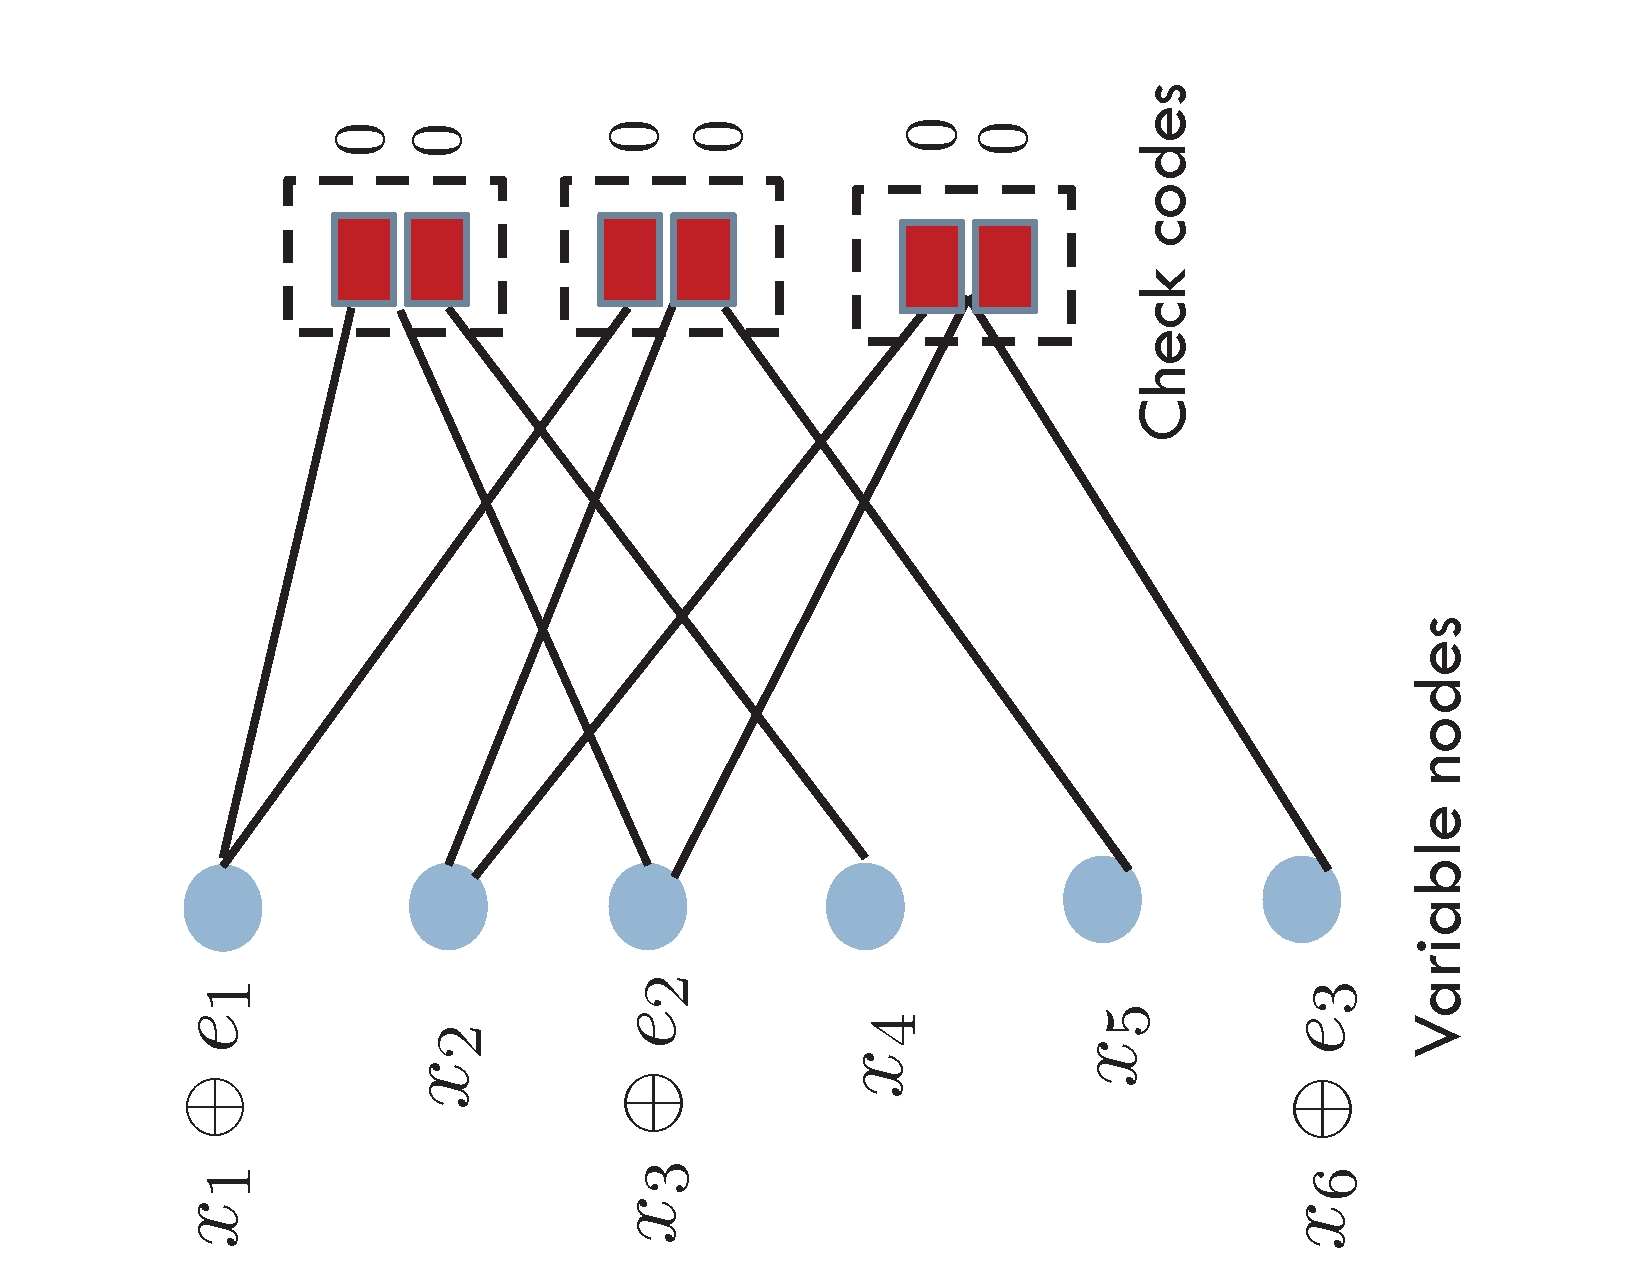
\includegraphics[width=2.0in,angle=-90]{./Figures/syndromesourcecoding2_1}
%\end{center}
%\begin{itemize}
%  \item $H \underline{x} = 0$
%  \item Receive - $\underline{r} = \underline{x} \oplus \underline{e}$
%  \item $H \underline{r} = H \underline{e} = \underline{y}$
%  \item Recover $\xv$ and sparse $\ev$
%\end{itemize}
%\column{0.5\textwidth}
%\begin{center}
%  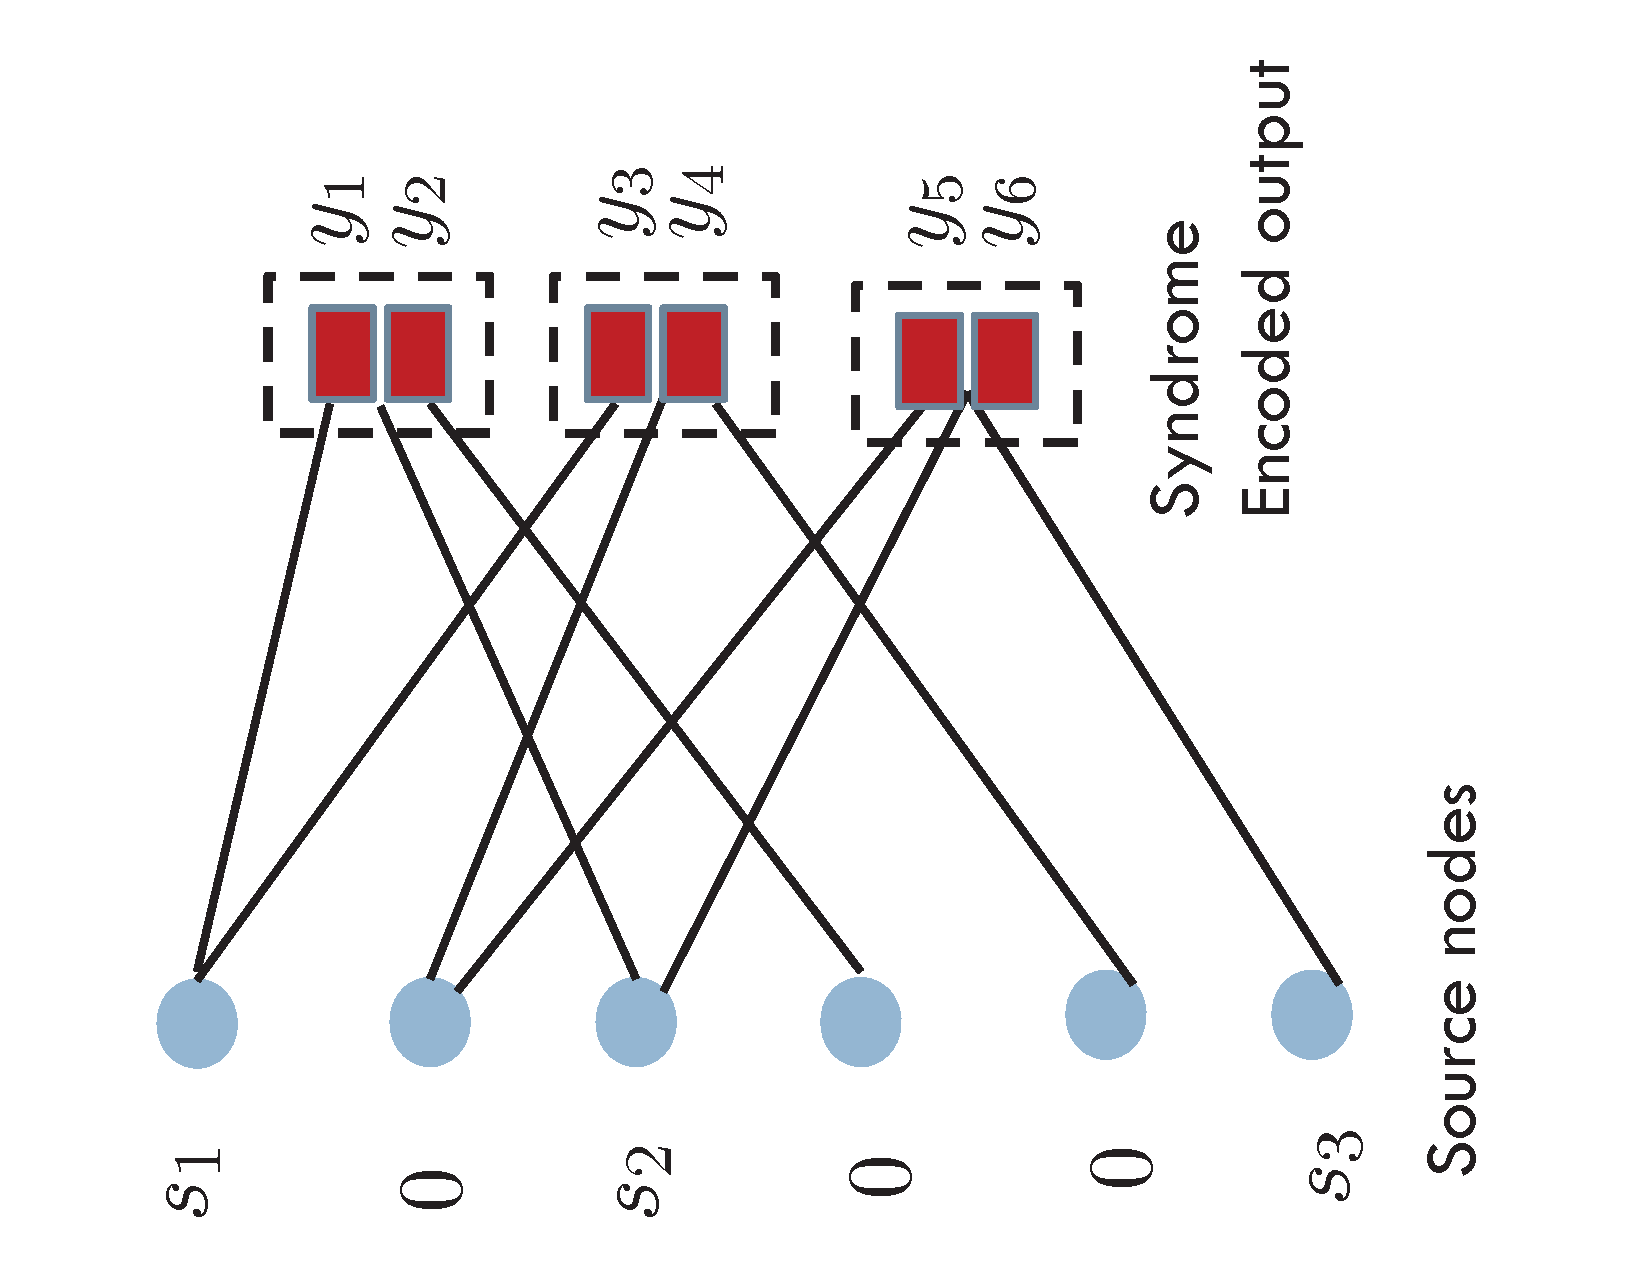
\includegraphics[width=2.0in,angle=-90]{./Figures/syndromesourcecoding2_2}
%\end{center}
%\begin{itemize}
%  \item $H \underline{s} = \underline{y}$
%  \item Set $\underline{r} = 0 $ (Let a genie add $\underline{x}$ to $\underline{r}$)
%  \item $\underline{y}$ is given to the decoder
%  \item Recover sparse $\sv$
%\end{itemize}
%\end{columns}
%\end{frame}
%------------------------------------------			
\begin{frame} \frametitle{Syndromes and decoding}
%-----------------------------------------------------			
\vspace*{-0.25in}
\begin{figure}[t]
			\centering
            \resizebox{4.0in}{!}{\begin{tikzpicture}

%A matrix
\draw [fill=cyan, opacity=.2,rotate=90, thick]  (0.1,4.35) node (v1) {} rectangle (3.9,-3.75) node (v2) {};
\draw [thick,rotate=90,red] (v1) rectangle (3.9,3.1);
\draw [thick,rotate=90,red] (0.1,3.1) rectangle (3.9,1.8) node (v7) {};
\draw [thick,rotate=90,red] (0.1,-2.45) node (v6) {} rectangle (v2);
\draw[thick,red]  (v6) rectangle (1.15,3.9);
\draw[thick,red]  (v7) rectangle (-0.55,0.1);

\node at (-0.45,-1.4) {\huge \color{red} $ \underset{ \color{blue} ( Parity  \ checks)}{H_{ m \times n} }$};

% X vector
\draw [ thick] (5.85,5) rectangle (6.85,6);
\draw [thick] (6.85,5) rectangle (5.85,4);
\draw [thick] (5.85,4) rectangle (6.85,3);
\draw [] (5.85,3) node (v4) {} rectangle (6.85,-0.1) node (v5) {};
\draw [thick] (5.85,-0.1) rectangle (6.85,-1.1);
\draw [thick] (5.85,-1.1) rectangle (6.85,-2.1) node (v8) {};
\node at (6.45,-3.4) {\huge \color{red}  $\underset{\tiny \color{blue} (code \ vector)}{c_{n \times 1 }} $};
\node at (6.35,1.6) {\Large \bf \vdots};

\draw [thick] (v4) rectangle (6.85,2.1);
\draw [thick] (v5) rectangle (5.85,0.8);

% delta-x vector
\draw [ thick, fill=green] (9.4,5) rectangle (10.4,6);
\draw [thick] (10.4,5) rectangle (9.4,4);
\draw [thick, fill=green] (9.4,4) rectangle (10.4,3);
\draw [] (9.4,3) node (v4) {} rectangle (10.4,-0.1) node (v5) {};
\draw [thick, fill=green] (9.4,-0.1) rectangle (10.4,-1.1);
\draw [thick] (9.4,-1.1) rectangle (10.4,-2.1);
\node at (10,-3.4) {\huge \color{red}  $\underset{\color{black}{t-sparse}}{\underset{\tiny \color{blue} (error \ vector)}{e}} $};
\node at (9.9,1.6) {\Large \bf \vdots};
\node at (4.8,2.1) {\bf \Huge $\times$};
\draw [thick] (v4) rectangle (10.4,2.1);
\draw [thick] (v5) rectangle (9.4,0.8);

\node at (8.2,2) {\Huge \bf $+$};

\node at (9.9,5.5) {\color{red} \huge $ e_i$ };
\node at (9.9,3.5) {\color{red} \huge $ e_j$};
\node at (9.9,-0.55) {\color{red} \huge $ e_t$};

% y







\node at (15.9,1.6) {\bf \vdots};

\node at (11.8,2) {\Huge = };
\node at (15.8,-0.65) {\color{red} \huge $y_{m \times 1}$};
\node [align=left, text width =3.5cm] at (16.5,-2.15) {\Large  \color{blue} Syndromes};

\node at (0.3,2.45) {\Huge \bf $\cdots$};



% b_k

\draw [thick] (15.4,4.1) node (v3) {} rectangle (16.4,3.1);
\draw [thick] (15.4,3.1) rectangle (16.4,2.1);
\draw [thick] (15.4,2.1) rectangle (16.4,1);
\draw [thick] (15.4,1) rectangle (16.4,0);
\draw[fill=red, opacity=0.2]  (v3) rectangle (16.4,0);
\node at (-1.35,1.6) { \color{blue}\Large  \bf  \vdots};

\draw [dashed,blue] (-4.35,3.9) rectangle (3.75,3);
\draw [dashed,blue] (-4.35,3) rectangle (3.75,2);
\draw[dashed,blue]  (v1) rectangle (3.75,1);
\node at (-3.85,4.5) {\huge \bf  \color{red} $h_1$};
\node at (-2.4,4.5) {\huge \bf \color{red} $h_2$};
\node at (-1.25,4.5) {\huge \bf  \color{red} $h_i$};
\node at (0.25,4.5) {\huge \bf  \color{red} $\cdots$};
\node at (1.8,4.5) {\huge \bf  \color{red} $h_{n-1}$};
\node at (3.15,4.5) {\huge \bf  \color{red} $h_n$};

\node at (9.9,4.55) {\large \bf \vdots};


\node at (13.45,2) {\bf \Huge $0$};
\node at (14.45,2) {\huge \bf +};

\draw [fill=orange, opacity=0.5] (v8) rectangle (5.85,6);
\end{tikzpicture} }
			%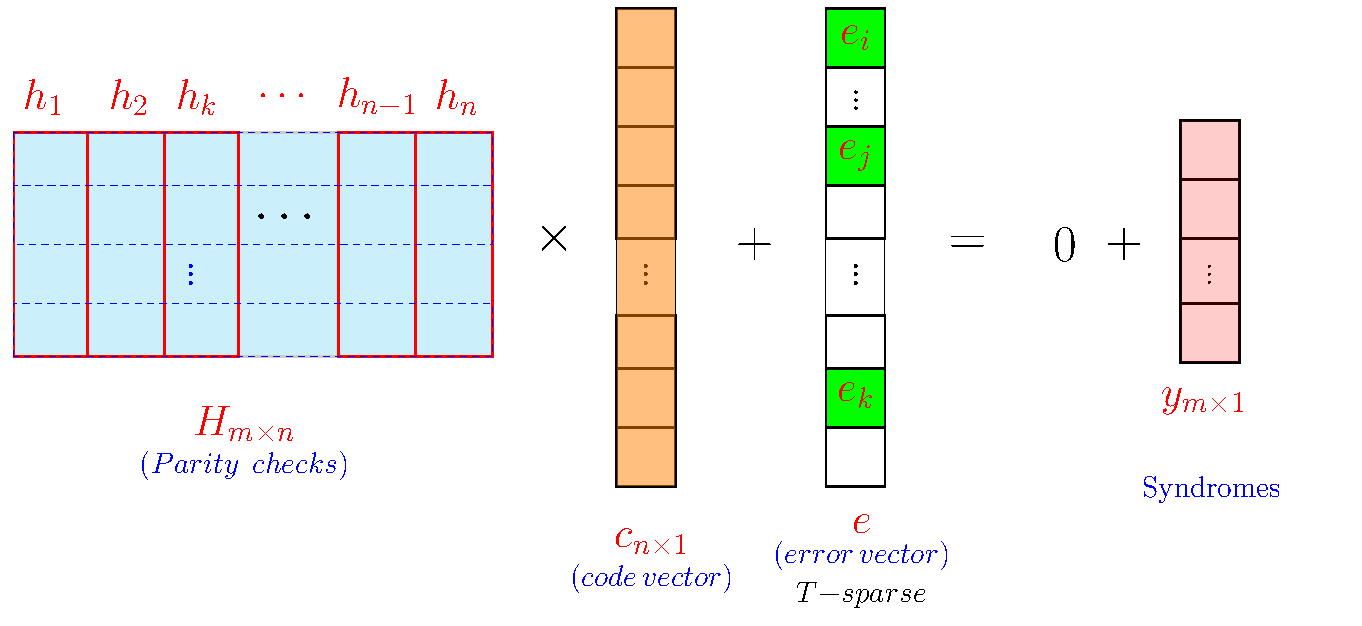
\includegraphics[width=4.0in]{./Figures/A_times_X_columns_coding.pdf}
		\end{figure}
\pause
\begin{itemize}
\item Syndrome : Linear combination of $\underline{h}_i$s, i.e., $\underline{y} = e_i \hv_i \oplus e_j \hv_j \oplus e_t \hv_t$
\item Decoding : Find min weight $\underline{e}$ : $\underline{y} = e_i \hv_i \oplus e_j \hv_j \oplus e_t \hv_t$
\end{itemize}
\pause
\begin{block}{\alert{Coding theory deals with the construction of $\mathbf{H}$ and efficient decoding algorithms, i.e., given a linear combination of the columns of $\mathbf{H}$, it develops tools to determine a sparse $\underline{e}$ }}\end{block}
\end{frame}
%------------------------------------------			
\begin{frame} \frametitle{Syndrome source coding}
%\begin{block}{Compression of a $p-$ary source}
%\[
%\begin{bmatrix}
%y_1\\
%\vdots\\
%y_m\\
%\end{bmatrix}
%=
%\begin{bmatrix}
%  1 & 1 & 1 & \ldots & 1 \\
%  1 & W & W^2 & \ldots & W^{n-1} \\
%  1 & W^2 & W^4 & \ldots & W^{2n-2} \\
%  \vdots & \vdots & \vdots & \vdots & \vdots \\
%  1 & W^{2t-1} & W^{4t-2} & \ldots & W^{(2t-1)(n-1)}\\
%\end{bmatrix}
%\begin{bmatrix}
%0\\
%\vdots\\
%x_1\\
%\vdots \\
%x_{k}\\
%\vdots\\
%0\\
%\end{bmatrix}
%\]
%\end{block}

\resizebox{4.0in}{!}{\begin{tikzpicture}

%A matrix
\begin{scope}[shift={(2,0)}]
\draw [fill=cyan, opacity=0.2,rotate=90, thick]  (0.1,4.35) node (v1) {} rectangle (3.9,-3.75) node (v2) {};
\draw [thick,rotate=90,red] (v1) rectangle (3.9,3.1);
\draw [thick,rotate=90,red] (0.1,3.1) rectangle (3.9,1.8) node (v7) {};
\draw [thick,rotate=90,red] (0.1,-2.45) node (v6) {} rectangle (v2);
\draw[thick,red]  (v6) rectangle (1.15,3.9);
\draw[thick,red]  (v7) rectangle (-0.55,0.1);
\node at (-0.45,-1.4) {\huge \color{red} $ \underset{ \color{blue} ( Parity  \ check \ matrix )}{H_{ m \times n} }$};
\node at (4.8,2.1) {\bf \Huge $\times$};
\node at (0.3,2.45) {\Huge \bf $\cdots$};
\node at (-1.35,1.6) { \color{blue}\Large  \bf  \vdots};
\draw [dashed,blue] (-4.35,3.9) rectangle (3.75,3);
\draw [dashed,blue] (-4.35,3) rectangle (3.75,2);
\draw[dashed,blue]  (v1) rectangle (3.75,1);
\node at (-3.85,4.5) {\huge \bf  \color{red} $h_1$};
\node at (-2.4,4.5) {\huge \bf \color{red} $h_2$};
\node at (-1.25,4.5) {\huge \bf  \color{red} $h_i$};
\node at (0.25,4.5) {\huge \bf  \color{red} $\cdots$};
\node at (1.8,4.5) {\huge \bf  \color{red} $h_{n-1}$};
\node at (3.15,4.5) {\huge \bf  \color{red} $h_n$};

\end{scope}










% X vector
%\draw [ thick] (5.85,5) rectangle (6.85,6);
%\draw [thick] (6.85,5) rectangle (5.85,4);
%\draw [thick] (5.85,4) rectangle (6.85,3);
%\draw [] (5.85,3) node (v4) {} rectangle (6.85,-0.1) node (v5) {};
%\draw [thick] (5.85,-0.1) rectangle (6.85,-1.1);
%\draw [thick] (5.85,-1.1) rectangle (6.85,-2.1) node (v8) {};
%\node at (6.45,-3.4) {\huge \color{red}  $\underset{\tiny \color{blue} (code \ vector)}{c_{n \times 1 }} $};
%\node at (6.35,1.6) {\Large \bf \vdots};
%
%\draw [thick] (v4) rectangle (6.85,2.1);
%\draw [thick] (v5) rectangle (5.85,0.8);

% delta-x vector
\draw [ thick, fill=green] (9.4,5) rectangle (10.4,6);
\draw [thick] (10.4,5) rectangle (9.4,4);
\draw [thick, fill=green] (9.4,4) rectangle (10.4,3);
\draw [] (9.4,3) node (v4) {} rectangle (10.4,-0.1) node (v5) {};
\draw [thick, fill=green] (9.4,-0.1) rectangle (10.4,-1.1);
\draw [thick] (9.4,-1.1) rectangle (10.4,-2.1);
\node at (10,-3.4) {\huge \color{red}  $\underset{\color{black}{t-sparse}}{\underset{\tiny \color{blue} (Source \ vector)}{x}} $};
\node at (9.9,1.6) {\Large \bf \vdots};

\draw [thick] (v4) rectangle (10.4,2.1);
\draw [thick] (v5) rectangle (9.4,0.8);

%\node at (8.2,2) {\Huge \bf $+$};

\node at (9.9,5.5) {\color{red} \huge $ x_1$ };
\node at (9.9,3.5) {\color{red} \huge $ x_i$};
\node at (9.9,-0.55) {\color{red} \huge $ x_t$};

% y

\begin{scope}[shift={(-1,0)}]
\node at (15.9,1.6) {\bf \vdots};
\node at (15.8,-0.65) {\color{red} \huge $y_{m \times 1}$};
\node [align=left, text width =3.5cm] at (16.5,-2) {\Large  \color{blue} Syndromes};
\draw [thick] (15.4,4.1) node (v3) {} rectangle (16.4,3.1);
\draw [thick] (15.4,3.1) rectangle (16.4,2.1);
\draw [thick] (15.4,2.1) rectangle (16.4,1);
\draw [thick] (15.4,1) rectangle (16.4,0);
\draw[fill=red, opacity=0.2]  (v3) rectangle (16.4,0);

\end{scope}


\node at (11.8,2) {\Huge = };







% b_k



















\node at (9.9,4.55) {\large \bf \vdots};


%\node at (13.45,2) {\bf \Huge $0$};
%\node at (14.45,2) {\huge \bf +};
%
%\draw [fill=orange, opacity=0.5] (v8) rectangle (5.85,6);


\end{tikzpicture}
}

\begin{block}{Compression of a sparse binary source}
\begin{itemize}
\item Compressed version is the syndrome $\yv$
\item Reconstruction is the same as decoding
\item Similar to the canonical sparse recovery problem
\end{itemize}
\end{block}
\end{frame}
%------------------------------------------------------------------------------
\begin{frame}\frametitle{Review of primitives}
\begin{itemize}
\item Idea of a check node or a measurement node which is a function of some symbols
\item Singleton detection - be able to identify one non-zero symbol
\item Peeling - if we know some symbols, be able to remove and adjust measurement
\end{itemize}
\end{frame}
%------------------------------------------------------------------------------
\begin{frame}{Application 3}
\end{frame}
%------------------------------------------------------
\begin{frame} \frametitle{Compressed sensing}
%-----------------------------------------------------
\vspace*{-0.2in}
\begin{figure}[t]
\centering
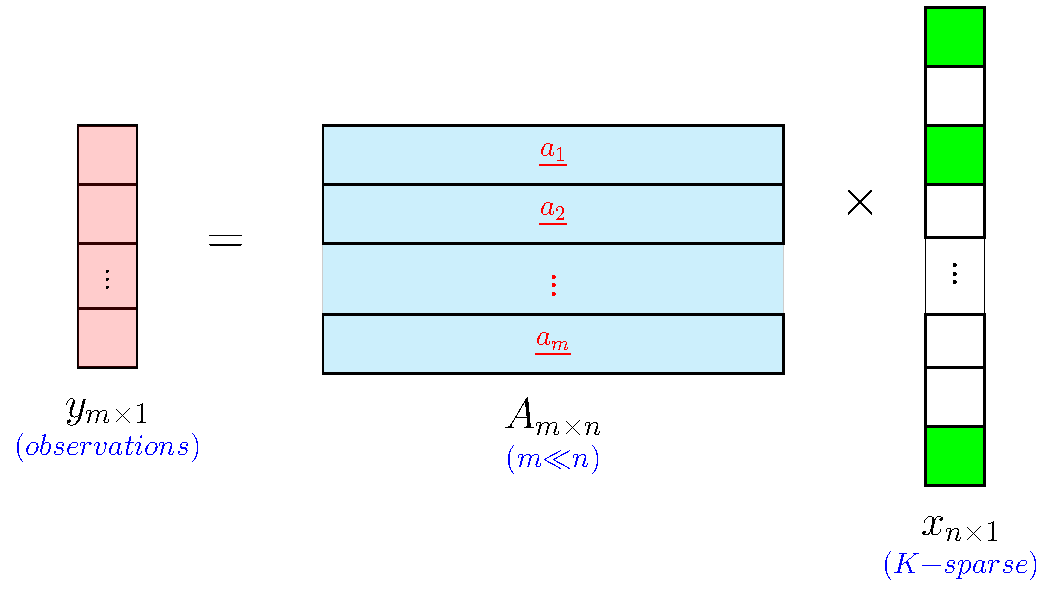
\includegraphics[width=2.75in]{./Figures/A_times_X_CS.pdf}
\end{figure}
\vspace*{-0.2in}
\begin{block}{Classical compressed sensing}
\begin{itemize}
\item $\xv$ is a $K$-sparse vector over $\mathbb{R}$ or $\mathbb{C}$
\item We `compress' $\xv$ by storing only $\yv = \mathbf{A} \ \xv$
\item Reconstruction - Solve $\hat{\xv} = \arg \min ||\zv||_0 : \yv = \mathbf{A} \zv$
\item CS - Solve $\hat{\xv} = \arg \min ||\zv||_1 : \yv = \mathbf{A} \zv$
\end{itemize}
\end{block}
\pause
\begin{block}{Coding theoretic approach - syndrome source coding over complex numbers}
\begin{itemize}

\item Sensing matrix $\mathbf{A} \Leftrightarrow $ Parity check matrix $\mathbf{H}$
\end{itemize}
\end{block}
\end{frame}		
%-------------------------------------------------------			
\begin{frame} \frametitle{Data stream computing}
%---------------------------------------------------------
\vspace*{-0.1in}
\begin{block}{Problem - consider a router in a large network}
\begin{itemize}
\item Count the number of packets from source $i$ to destination $j$, say $x_{ij}$
\item Data vector is huge, $n = 2^{64}$
\item Heavy hitters - only a few of them are large
\end{itemize}
\end{block}

\vspace*{-0.1in}
\begin{figure}[t]
		\centering
		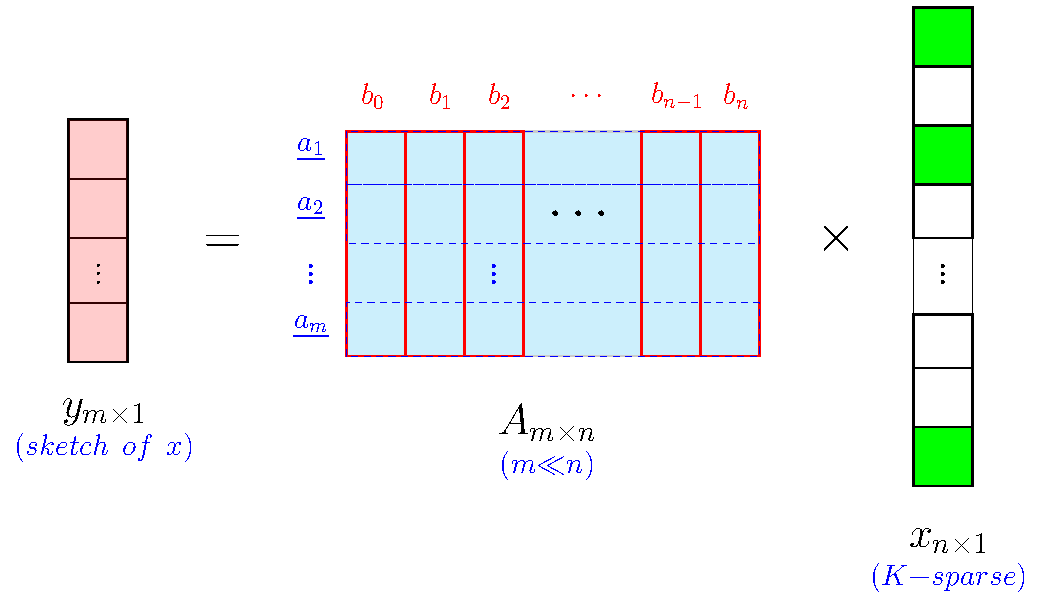
\includegraphics[width=3.0in]{./Figures/A_times_X_columns.pdf}
	\end{figure}
\vspace*{-0.2in}
\begin{block}{Keep only a low dimensional ($m \ll n$) sketch of $x$}	
\begin{itemize}
\item {\color{blue}$\yv_{m \times 1} = \mathbf{A} \xv \Leftrightarrow$} Syndrome, $x_{i,j} \in \mathbb{Z}^+$
\item Reconstruction is same as decoding
\end{itemize}	
\end{block}	

\end{frame}

%------------------------------------------------------------------
\begin{frame}\frametitle{Incremental updates}

	\begin{figure}[t]
		\centering
		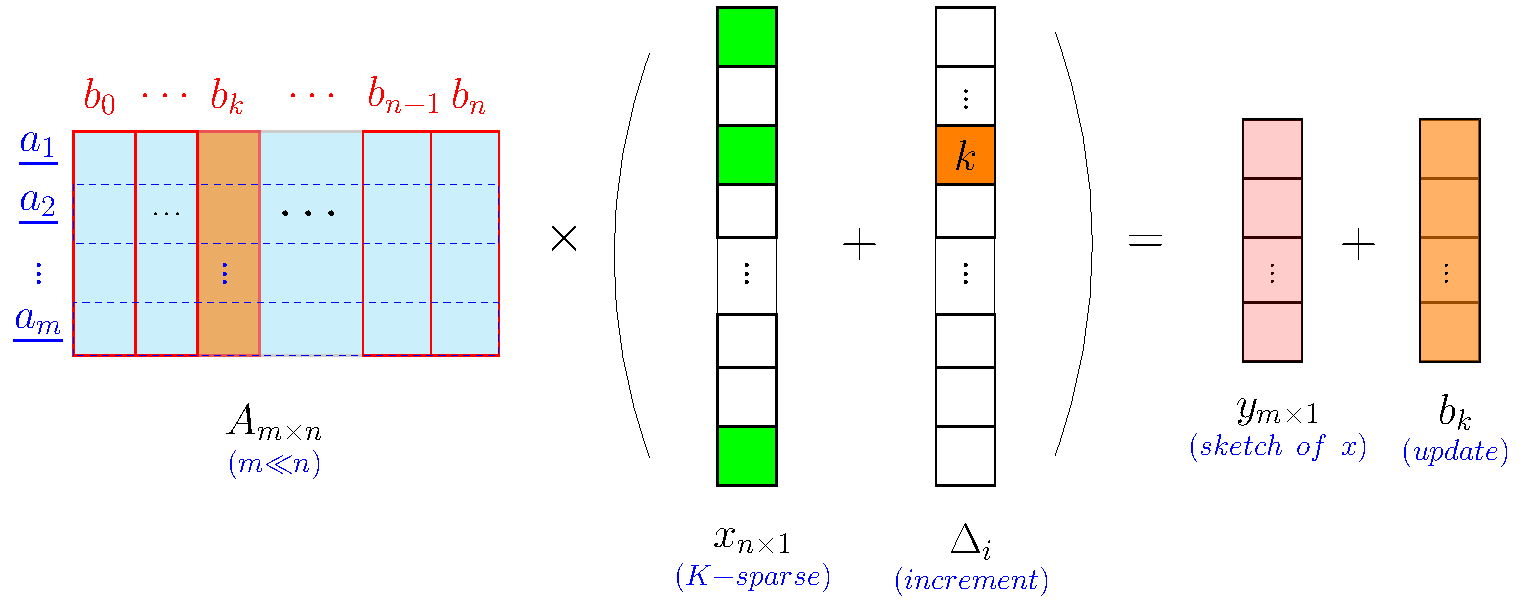
\includegraphics[width=4.7in]{./Figures/A_times_X_columns_Stream_inc.pdf}
	\end{figure}

\begin{block}{}

Sketch $y$ {\color{blue} supports incremental updates} to $x$ as the sketching procedure is linear. \\
\centering{\color{blue}$x+ \Delta_i \rightarrow y + A\Delta_i$}\\ (adding $i$th column vector of $A$ to existing sketch)

\end{block}				
	
	
%								\begin{block}{Objective}
%					
%					\begin{itemize}
%						
%						\item Design the {\color{blue}sketching matrix} $A$ that offers {\color{blue} high compression rates} (smaller $m$)
%						\item Design a {\color{blue} less-complex decoding algorithm} to recover the sparse approximation of $x$ from $Ax$
%					\end{itemize}
%				\end{block}

	
\end{frame}

%------------------------------------------------------------------

%\begin{frame}\frametitle{Making the connection explicit}			
%
%\begin{center}
%	\begin{tabular}{|c|c|c|}
%\hline
%		\alert{Coding} & $\Leftrightarrow$ & \alert{Compressed sensing} \\
%\hline
%		Parity check matrix & $\Leftrightarrow$ & Sensing matrix \\
%\hline
%		Error locations & $\Leftrightarrow$ & Non-zero coefficients \\
%\hline
%        $k$-error correcting code & $\Leftrightarrow$ & $k$-sparse recovery \\
%\hline
%		Syndromes & $\Leftrightarrow$ & Measurements/Sketch \\
%\hline
%        Symbols from $\mathbb{F}_q$ & $\Leftrightarrow$ & Symbols from $\mathbb{R}$ or $\mathbb{C}$ \\
%\hline
%		Decoding & $\Leftrightarrow$ & Sparse recovery \\
%\hline
%
%	\end{tabular}
%\end{center}			
%\end{frame}
%------------------------------------------------------
\begin{frame} \frametitle{Compressed Sensing (Li, Ramchandran '14)}
%-----------------------------------------------------
\vspace*{-0.5in}
    \begin{columns}
    \column{0.45\textwidth}
    \begin{figure}[t]
    \centering
    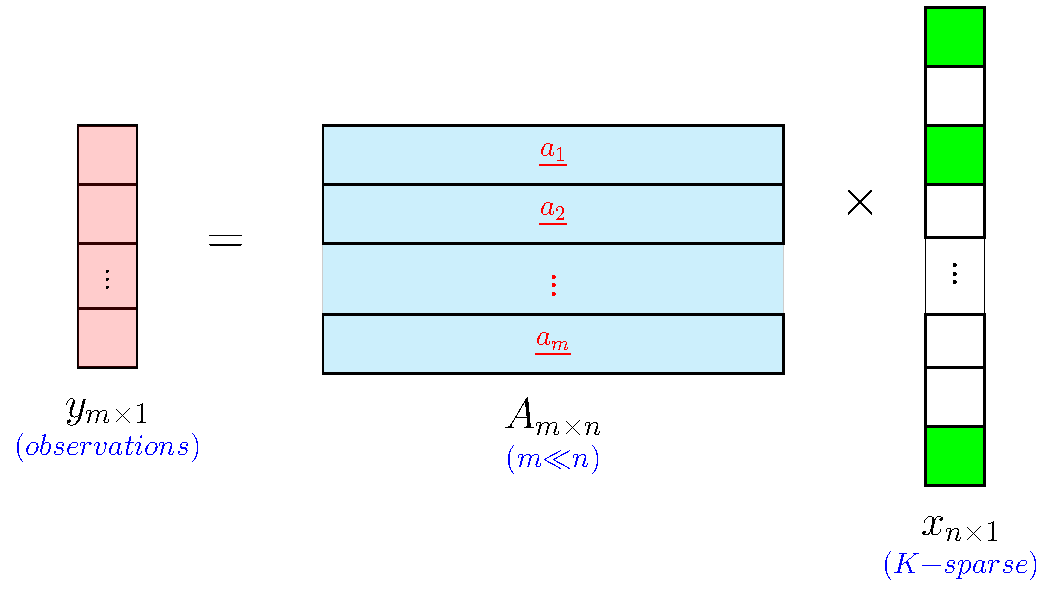
\includegraphics[width=2.5in]{./Figures/A_times_X_CS.pdf}
    \end{figure}
    \column{0.45\textwidth}
        \begin{figure}[t]
        \centering
        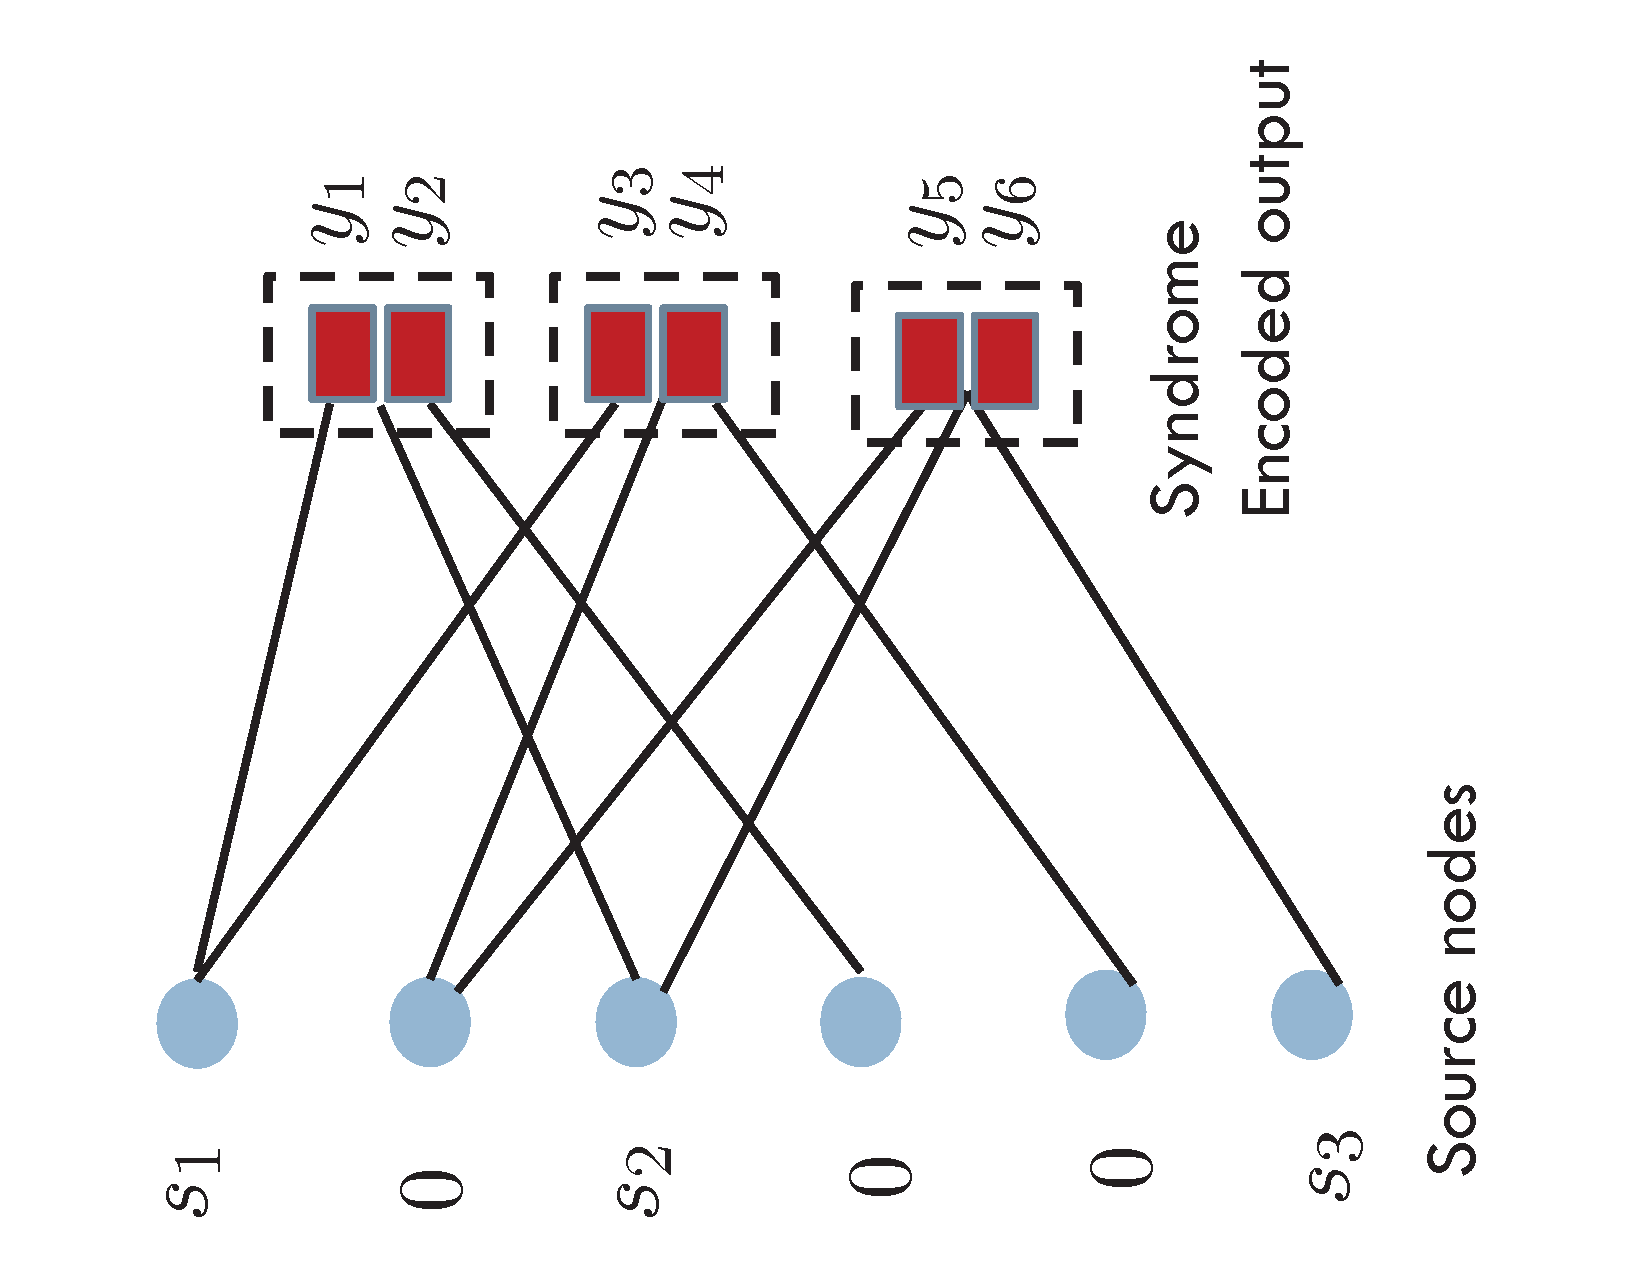
\includegraphics[width=1.75in,angle=-90]{./Figures/syndromesourcecoding2_2}
        \end{figure}
    \end{columns}

			\begin{block}{Sketching matrix ($A_{m\times n}$)}
				\centering
				$A_{m \times n}  = \underset{\color{blue} (d-left \ regular \ Graph)}{\bf H_{\frac{m}{2} \times n}} {\Large \bf \color{red} \otimes} \underset{\color{blue} (Singleton \ identifier)}{\bf B_{2 \times n}}$ \\
				
				\[ {\bf B} = \begin{bmatrix}
				1 & 1 & 1 & \cdots & 1\\
				1 & W & W^2 & \cdots & W^{n-1}
				\end{bmatrix} \ \  \alert{W = e^{j \frac{2\pi}{n}}} \]	
			\end{block}
\end{frame}

\begin{frame} \frametitle{Main results for compressed sensing}


%			\begin{block}{Singleton detection}
%					\begin{itemize}
%                    \item $y_i$ - $i$th observation is singleton if {\color{blue}$y_{i}[1]=x[l], \ y_{i}[2] = x[l]W^l $ }
%						%\item Singleton condition: { \color{blue} $\mid y_{i}[1] \mid \ =  \ \mid y_{i}[2] \mid $ } and ${\color{blue} \angle \frac {y_i[2]}{y_i[1]} \mod{ \frac{2 \pi}{n}} = 0}$
%					\item The position of non-zero component $\color{blue} l =  \frac{n}{2 \pi}\angle \frac {y_i[2]}{y_i[1]}$
%					\item Value of the participating non-zero coefficient {\color{blue} $: y_i[1]$}
%					\end{itemize}
%			\end{block}

\begin{block}{Noiseless case}
\begin{itemize}
\item Samples : $2K$ versus Info-theoretic limit $K+1$
\item Computations: $O(K)$ versus $O(K^2)$
\item If $K = O(n^\delta)$, small price to pay in terms of samples
\end{itemize}
\end{block}

\begin{block}{Noisy case}
\begin{itemize}
\item Sample: $O(k \log^{1.{3}^{.}} n)$ vs limit: $O(k \log(n/k))$ necessary and sufficient
\item Computations: $O(k \log^{1.{3}^{.}} n)$
\end{itemize}
\end{block}
\pause
\begin{block}{Vem, Thenkarai Janakiraman, N. ITW'16}
\begin{itemize}
\item Sample: $O(k \log^{1.{3}^{.}} (n/k))$ vs limit: $O(k \log(n/k))$ necessary and sufficient
\item Computations: $O(k \log^{1.{3}^{.}} (n/k))$
\end{itemize}
\end{block}
\end{frame}

%------------------------------------------------------------------

\begin{frame}
	\frametitle{Group Testing (Lee, Pedarsani, Ramchandran '15)}
	\begin{figure}[t]
		\centering
		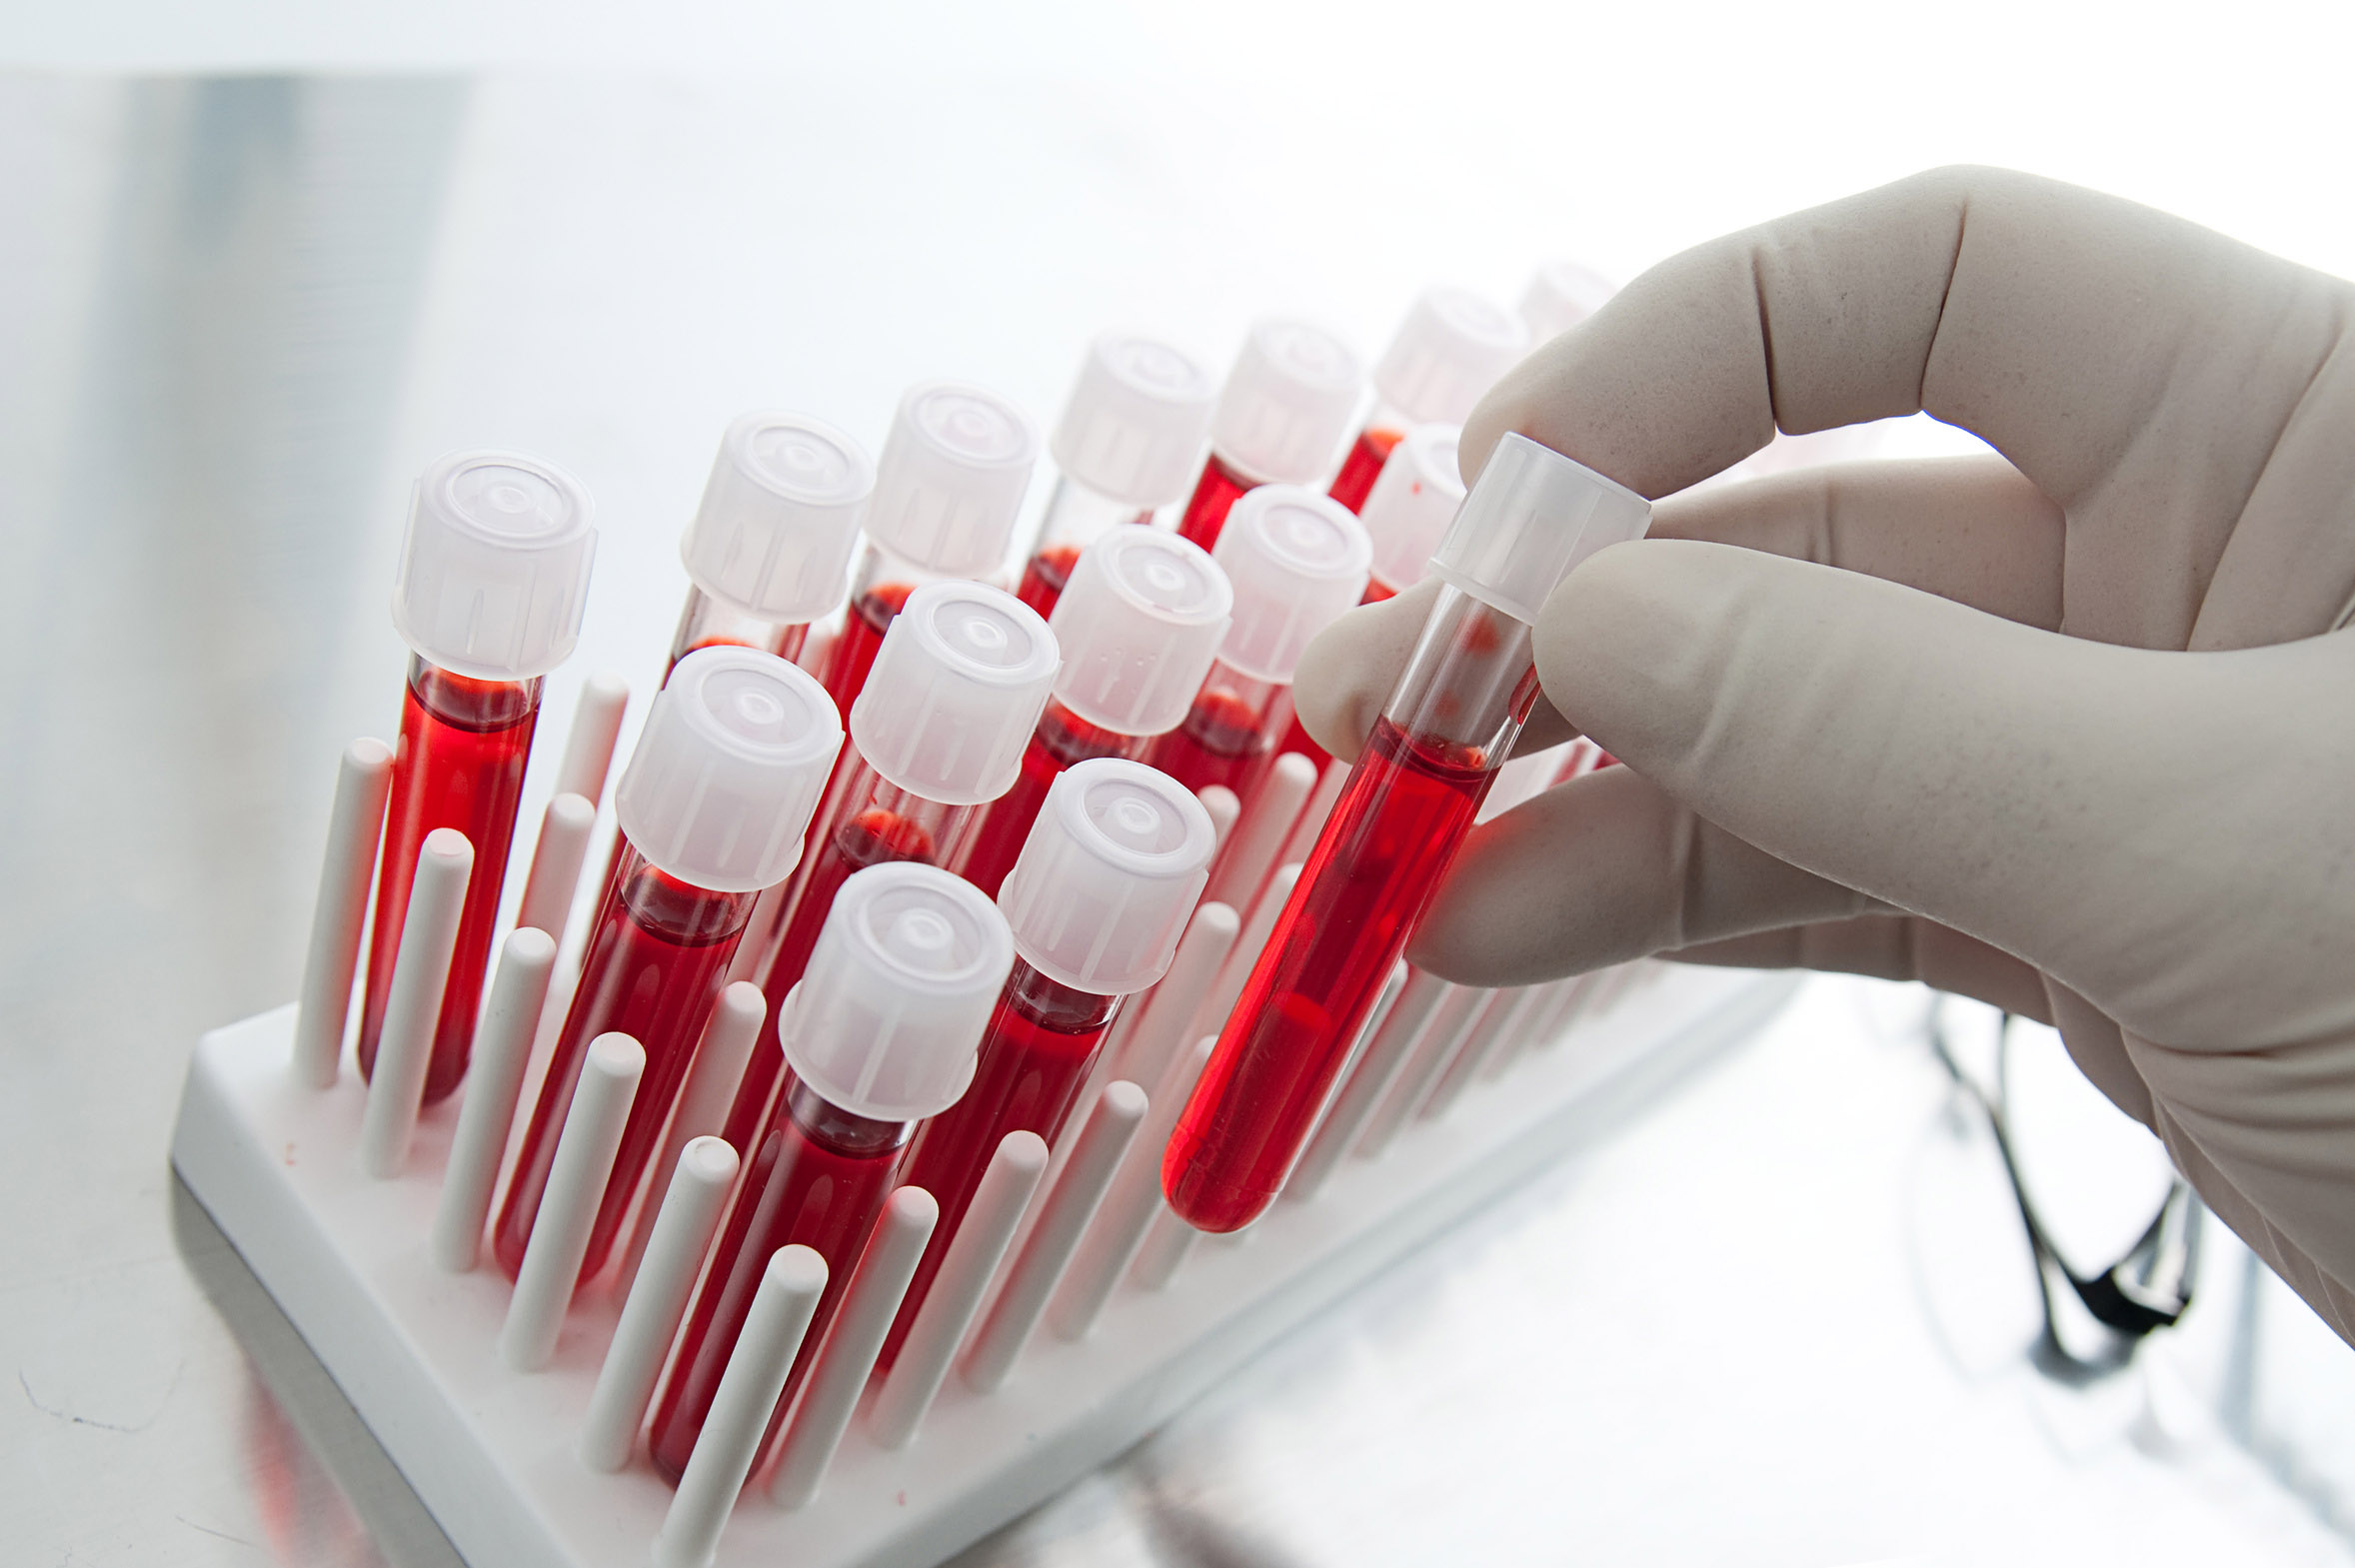
\includegraphics[width=1.8in]{./Figures/grouptest_testubes.jpg}
	\end{figure}

\begin{itemize}
	\item II World War - detect all soldiers with syphilis
	\item Tests performed on efficiently pooled groups of items
	\item Least no. of tests ($m$) to identify $k$ defective items from $n$ items
\end{itemize}	

\end{frame}
%------------------------------------------------------------------
\begin{frame}\frametitle{Group Testing}

\alert{Example}
\vspace{-0.3in}
	\begin{figure}[t]
		\centering
		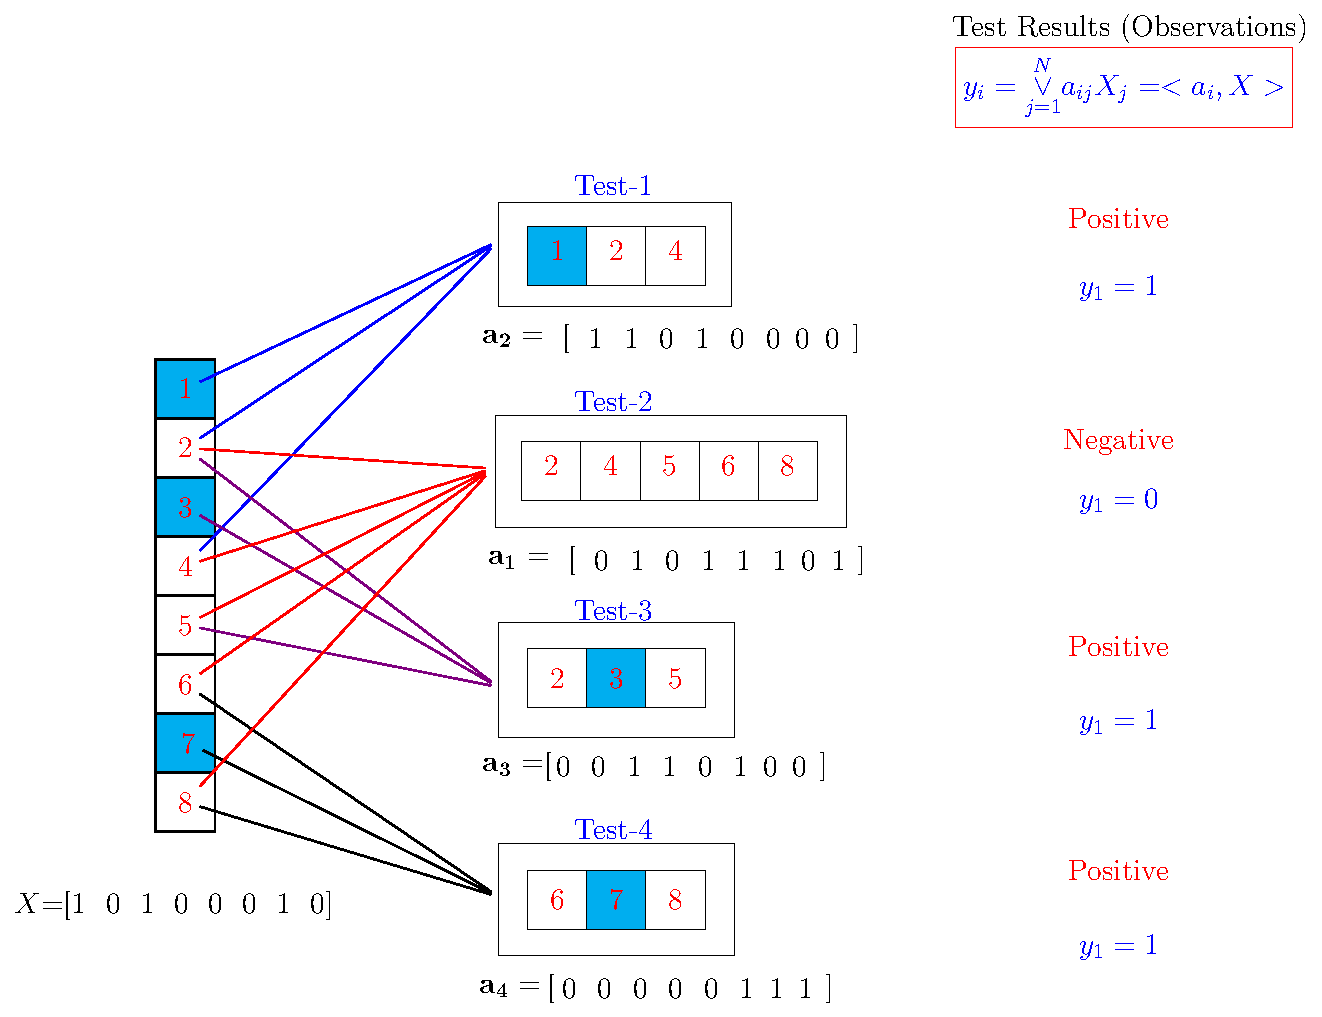
\includegraphics[width=4.2in]{./Figures/grouptesting_example.pdf}
	\end{figure}

\end{frame}


\begin{frame} \frametitle{Group Testing}

\begin{figure}[t]
\centering
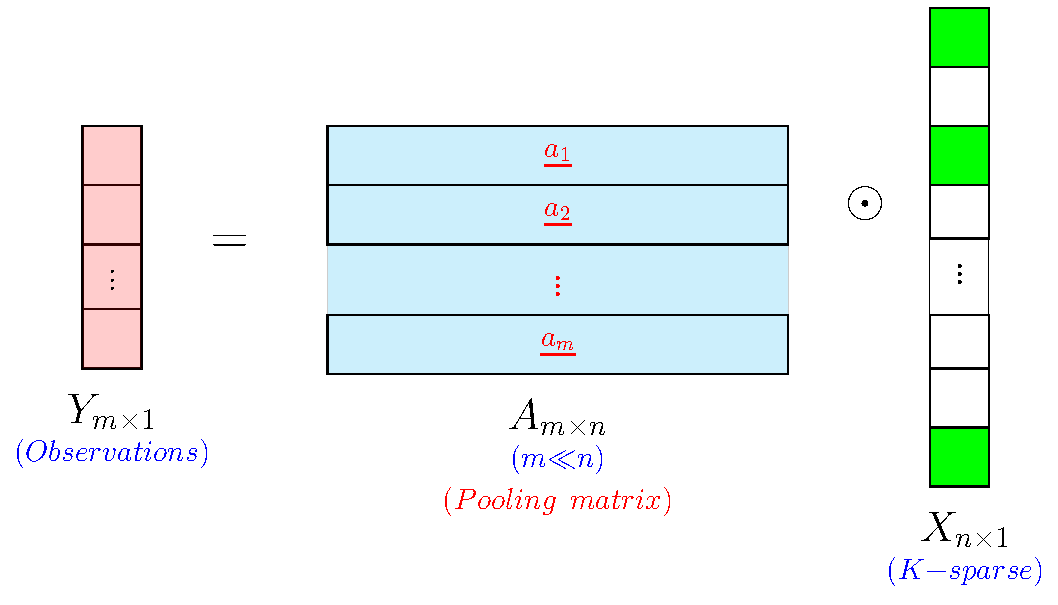
\includegraphics[width=3.4in]{./Figures/A_times_X_group_testing.pdf}
\end{figure}



\begin{block}
%		{
		%\[ \small \underset{\color{blue} (Pooling \ matrix)}{A_{m \times N} } =  \begin{bmatrix}
%			\bf{a_1} \\
%			\bf{a_2}  \\
%			\vdots  \\
%			\bf{a_m}
%			\end{bmatrix} \] }
		
		
	
	{
		\[ \small \underset{\color{blue}(Observation \ vector)}{Y_{m \times 1}} = A \odot X = \begin{bmatrix}
		{<a_1,X>} \\
		{<a_2,X>}  \\
		\vdots  \\
		{<a_m,X>}
		\end{bmatrix} \ \   <a_i , X> = \overset{N}{\underset{j=1 }{\vee}} a_{ij}X_j  \] }
		
\end{block}

%------------------------ commented ---------------------			
%		\begin{block}{Objective}
%			\begin{itemize}
%				\small
%				\item Design the {\color{blue}pooling matrix} ($A_{m \times N}$) with $m$ as low as possible,
%				\item Determine a {\color{blue}less-complex decoding procedure} to find the positions of 1s in $X$ using $Y$.
%			\end{itemize}
%		\end{block}

%--------------------------------------------------------
\end{frame}

%--------------------------------------------------------
	  \begin{frame}\frametitle{Group Testing}
				\begin{block}{Singleton detection}
				
				{ \tiny
		\[	\begin{bmatrix}
		H_1 \\
		\overline{H_1}
\end{bmatrix}	 =  \begin{bmatrix}
					\bf{b_1} & \bf{b_2} & \bf{b_3} & \cdots & \bf{b_{n-1}}\\
				   	\bf{\overline{b_1}} & \bf{\overline{b_2}} & \bf{\overline{b_3}} & \cdots & \bf{\overline{b_{n-1}}} \end{bmatrix} = \begin{bmatrix}
		0      & 0   & 0 & \cdots & 1 &  1 \\
		0      & 0   & 0 & \cdots & 1 &  1  \\
		\vdots & \vdots & \vdots & \ddots & \vdots & \vdots \\
		0      & 0   & 1 & \cdots & 1 &  1  \\
		0      & 1   & 0 & \cdots & 0 &  1  \\
		-- & -- & -- & -- & -- & --  \\
        1      & 1   & 1 & \cdots & 0 &  0 \\
		1      & 1   & 1 & \cdots & 0 &  0  \\
		\vdots & \vdots & \vdots & \ddots & \vdots & \vdots \\
		1      & 1   & 0 & \cdots & 0 &  0  \\
		1      & 0   & 1 & \cdots & 1 &  0  \\
		\end{bmatrix}
				   				   	 \]}
\alert{Note:} If a checknode is a singleton, with $i$th bit-node participating, then the observation vector is the $i$th column of $A$.

\begin{itemize}
\item Singleton - if the {\color{blue}weight of first two observation} vectors together is{ \ \color{blue} $L$}.
\item {\color{blue}Position} of the defective item is - {\color{blue} decimal value of the 1st observation vector}.
\end{itemize}    				
\end{block}					
					
\end{frame}
%---------------------------------------------------------------------------------
	  \begin{frame}\frametitle{Group Testing}
\vspace*{-0.1in}
  \begin{block}{Measurement matrix ($A_{m\times n}$)}
  {\centering
  $A_{m \times n}  = \underset{\color{blue} (d-left \ regular \ Graph)}{\bf G_{\frac{m}{6} \times n}} {\Large \bf \color{red} \otimes} \underset{\color{blue} (Singleton \ identifier)}{\bf H_{6 \times n}}$ \\
  \vspace{6pt}
  Let, $\bf{b_i}$ denote the {\color{blue}$L$-bits binary representation of the integer $i-1$}, $L=\lceil \log_2{n} \rceil$.
   {\small \[ H = \begin{bmatrix}
					\bf{b_1} & \bf{b_2} & \bf{b_3} & \cdots & \bf{b_{n-1}}\\
				   	\bf{\overline{b_1}} & \bf{\overline{b_2}} & \bf{\overline{b_3}} & \cdots & \bf{\overline{b_{n-1}}}\\
					\bf{b_{i_1}} & \bf{b_{i_2}} & \bf{b_{i_3}} & \cdots & \bf{b_{i_{n-1}}}\\
				   	\bf{\overline{b_{i_1}}} & \bf{\overline{b_{i_2}}} & \bf{\overline{b_{i_3}}} & \cdots & \bf{\overline{b_{i_{n-1}}}}\\
				   	
					\bf{b_{j_1}} & \bf{b_{j_2}} & \bf{b_{j_3}} & \cdots & \bf{b_{j_{n-1}}}\\
				   	\bf{\overline{b_{j_1}}} & \bf{\overline{b_{j_2}}} & \bf{\overline{b_{j_3}}} & \cdots & \bf{\overline{b_{j_{n-1}}}} \end{bmatrix} \]
$s_1=(i_1, i_2, \cdots, i_{n-1})$ and $s_2=(j_1, j_2, \cdots, j_{n-1})$ are permutations }}
 \end{block}

%\begin{block}{Main result}
%With {\color{blue} $m = 6C(\epsilon ) K log_2{n}$}, this decoding procedure can recover atleast $(1-\epsilon)K$ defective items with high probability
%\end{block}
\begin{block}{Decoding procedure}
\begin{itemize}
\item  Identify and decodes singletons using weights of the observation vector
\item Identify and resolve doubletons by guessing to satisfy the first pair of observation vectors and checking if the guess satisfies the other two pairs of observations
\item The iteration continues until no doubletons can be resolved
\end{itemize}

\end{block}

     \end{frame}



%\begin{frame} \frametitle{Group Testing}
%\begin{block}{Decoding procedure}
%\begin{itemize}
%\item  Identify and decodes singletons using weights of the observation vector
%\item Identify and resolve doubletons by guessing to satisfy the first pair of observation vectors and checking if the guess satisfies the other two pairs of observations
%\item The iteration continues until no doubletons can be resolved
%\end{itemize}
%
%\end{block}
%
%\end{frame}

\begin{frame} \frametitle{Main results for group testing}

\begin{block}{Non-adaptive Group Testing (Noiseless and Noisy)}
\begin{itemize}
\item Recovers $(1-\epsilon)k$ items with h.p.
\item Samples: $m = O(k \log_2 n)$ \ \ versus limit: $\Theta(k \log( \frac{n}{k} ))$
\item Computational complexity: $O(k \log n)$  (order optimal)
\end{itemize}
\end{block}
%\pause
%\begin{block}{Adaptive case}
%\begin{itemize}
%\item Don't know the results exactly
%\item Seems similar to coding with feedback
%\end{itemize}
%\end{block}

\end{frame}
%--------------------------------------------------------------------------
\begin{frame} \frametitle{Compressive Phase Retrieval}



\begin{figure}[t]
\centering
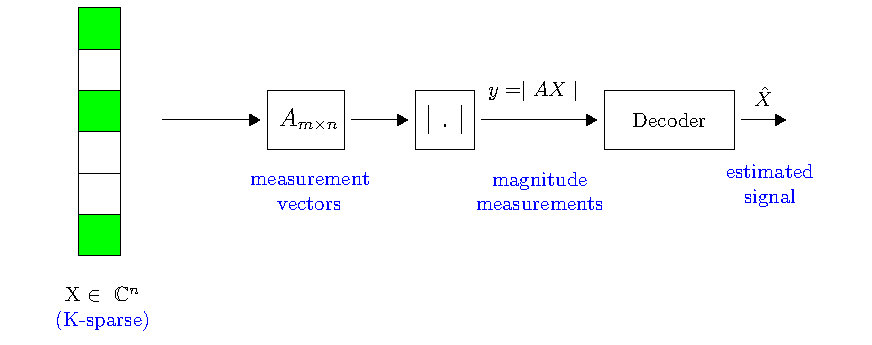
\includegraphics[width=3.6in]{./Figures/phase_retrieval.pdf}
\end{figure}

\pause		
\vspace{-.25in}
\begin{figure}[t]
\centering
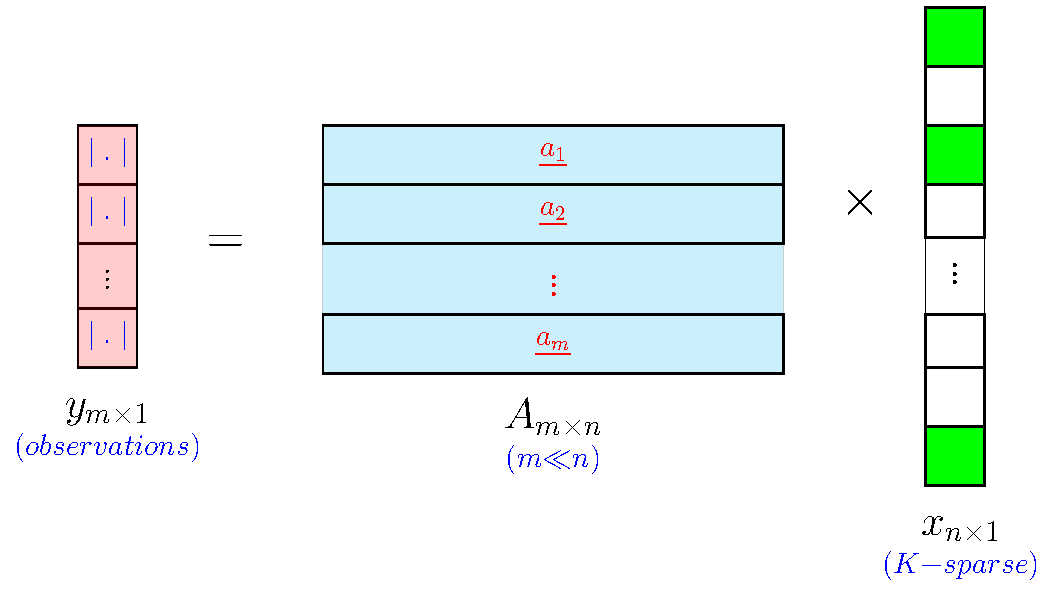
\includegraphics[width=3.1in]{./Figures/A_times_X_phase_retrieval.pdf}
\end{figure}
\end{frame}	
%---------------------------------------				
%		\begin{block}{}
%		\alert{Objective:} \begin{itemize}
%				\item Design the measurement matrix ($A_{m\times n}$) with $m$ as small as possible.
%				\item Design a less complex decoder to retrieve the $K$ non-zero elements (with phase) of $X$ from $\mid AX \mid$.
%			\end{itemize}
%		\end{block}		
%----------------------------------------------------		
\begin{frame}{Conclusion}
\begin{itemize}
  \item Review of a simple message passing decoder called the peeling decoder
  \item Density evolution as a tool to analyze its asymptotic performance
  \item Applications 
    \begin{itemize}
      \item Massive uncoordinated multiple access
      \item Sparse Fourier transform computation
      \item Compressed sensing type sparse recovery problems
    \end{itemize}
\end{itemize}
\end{frame}
	